%!TEX root = thesis.tex
% a related work section in which the relevant literature is presented and linked to the project;
\chapter{Related work}
\label{chap:rw}
A number of research topics are relevant for this thesis: how to use existing standards for publishing sensor data to the semantic web, developing ontologies that are suitable for many different kinds of sensor data and how to aggregate sensor data based on features-of-interest and time. This chapter discusses the recent relevant literature on these topics.     

\section{Sensor data catalogue service}
The \ac{sor} is "a web service interface for managing the definitions of phenomena measured by sensors as well as exploring semantic relationships between these phenomena" \cite[p. vi]{SW:OGC4}. This is a web service developed by \ac{ogc} to enable semantic reasoning on sensor networks, especially concerning phenomenon definitions. This should make it easier to discover sensors that observe a certain phenomenon and to interpret sensor data.

\cite{SW:OGC3} 

\section{Semantic sensor data middleware}
\cite{SSW:Henson} and \cite{SSW:Pschorr} suggest adding semantic annotations to a \ac{sos} which they call \ac{semsos}. In \ac{semsos} the raw sensor data goes through a process of semantic annotating before it can be requested with a \ac{sos} service. The retrieved data is still an \ac{xml} document, but with embedded semantic terminology as defined in an ontology model. The data retrieved from \ac{semsos} is therefore semantically enriched.  

\cite{SSW:Janowicz} has specified a method that uses a \ac{rest}ful proxy as a fa\c{c}ade for \ac{sos}. When a specific \ac{uri} is requested the so-called \ac{sel} translates this to a \ac{sos} request, fetches the data and translates the results back to \ac{rdf}. In this method the sensor data is converted to \ac{rdf} on-the-fly. This allows the data to be interpreted by both humans and machines.  

\cite{SSW:Atkinson} have identified that "distributed heterogeneous data sources are a necessary reality in the case of widespread
phenomena with multiple stakeholder perspectives" \cite[p.129]{SSW:Atkinson}. Therefore, they propose that methods should be developed to move away from the traditional dataset centric approaches and towards using linked data for cataloguing. This has the potential to bring together data and knowledge from different areas of research about the same (or similar) features-of-interest. It is also argued that using both linked data services and data-specific services could ease the transition into the linked data world.  

\section{Sensor data ontologies}
\paragraph{Semantic sensor network ontology} \mbox{}\\
 \ac{w3c} has developed an ontology for sensors and observations called the \ac{ssno}. This ontology aims to address semantic interoperability on top of the syntactic operability that the \ac{swe} standards provide. To accommodate different definitions of the same concepts the broadest definitions have been used. Depending on the interpretation these can be further defined with subconcepts. The \ac{ssno} is based on the stimulus-sensor-observation pattern, describing the relations between a sensor, a stimulus and observations (figure \ref{fig:sens-stim-obs}). Sensors are defined as "physical objects ... that observe, transforming incoming stimuli ... into another, often digital, representation", stimuli are defined as "changes or states ... in an environment that a sensor can detect and use to measure a property" and observations are defined as "contexts for interpreting incoming stimuli and fixing parameters such as time and location" \cite[p 28]{SSW:SSN_incubatorGroup}. The ontology can be used to model sensor networks from four different perspectives (sensor, observation, system, and feature \& property), which have been discussed together with additional relevant concepts.

\begin{figure}
	\centering
	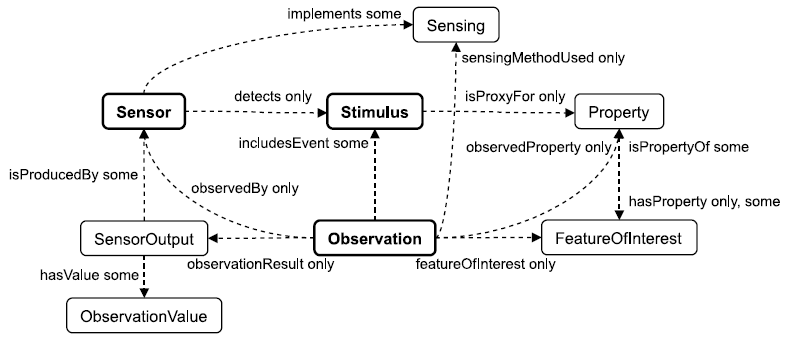
\includegraphics[width=1\linewidth]{figs/sens_stim_obs.png}
	\caption{The stimulus–sensor–observation pattern \cite[p. 28]{SSW:SSN_incubatorGroup}}
	\label{fig:sens-stim-obs}
\end{figure}

\paragraph{Observation capability metadata model} \mbox{}\\
\cite{SW:Hu} have reviewed a number of metadata models (including \ac{sensorml} and \ac{ssno}) for the use of earth observation (including remote sensing). They argue that all of the current metadata models are not sufficient for sensor data discovery. This conclusion is based on an evaluation of six criteria. Three steps have been identified in the process of obtaining relevant sensor data for earth observation, which have been used to derive criteria for their evaluation framework. These steps are sensor filtration, sensor optimisation and sensor dispatch. The filtration of sensors should result in a set of sensors that meets the requirements of the application: it should measure the right phenomenon, be active, be inside the spatial and temporal range, and have a certain sample interval. In sensor optimisation the selected sensors should be combined to complement or enhance each other. To do this, the observation quality, coverage and application is relevant. In the last step - sensor dispatch - the data should be retrieved, stored transmitted. In every evaluated model sensors can describe in different ways or only partially, which affects the outcome of the sensor dispatch. 

Therefore, a metadata model is proposed that "reuses and extends the existing sensor observation-related metadata standards" \cite[p. 10546]{SW:Hu}. It is composed of five modules: observation breadth, observation depth, observation frequency, observation quality and observation data. They should be derived from metadata elements described using the Dublin Core metadata element set. These five modules can then be formalized following the \ac{sensorml} schema which can be queried by users via the 'Unified Sensor Capability Description Model-based Engine' (figure \ref{fig:Hu}). 

\begin{figure}
	\centering
	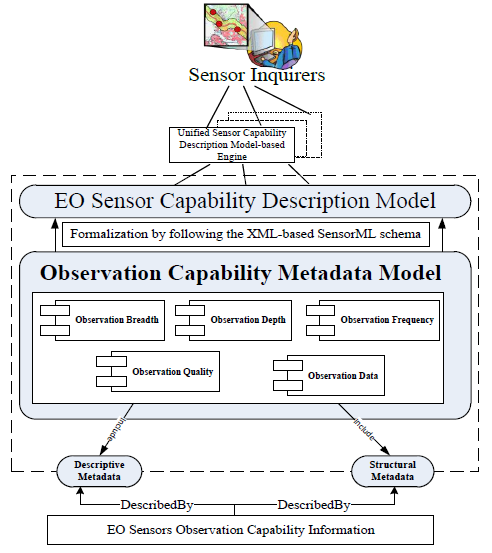
\includegraphics[width=0.8\linewidth]{figs/hu.png}
	\caption{Architecture of the sensor discovery system \cite[p. 10553]{SW:Hu}}
	\label{fig:Hu}
\end{figure}

\paragraph{Om-lite \& sam-lite ontologies} \mbox{}\\
\cite{SSW:Cox4} has been working on a new semantic ontology based on \ac{om}. Previous efforts, such as the \ac{ssno} have been using pre-existing ontologies and frameworks. However, there are already many linked data ontologies that could be useful for describing observation metadata, such as space and time concepts. Also, the \ac{ssno} does not take sampling features into account. The proposed om-lite ontology defines the concepts from \ac{om} regarding observations, while the sam-lite defines the sampling feature concepts. The author also provides a mapping of the \ac{ssno} to om-lite.

\cite{SSW:Cox4} also describes how the PROV ontology \cite{LD:PROV} can be directly used inside om-lite. The PROV ontology is "concerned with the production and transformation of Entities through time-bounded Activities, under the influence or control of Agents" \cite[p. 12]{SSW:Cox3}. This is a very convenient ontology to model real world entities, such as sensors, observation processes and sampling processes.  
 
\section{Sensor data aggregation}
\cite{SSW:Stasch} propose to aggregate sensor data based on the geometry of sampling features. \cite{SSW:Stasch3} proposes a \ac{wps} that takes sensor data right from a \ac{sos} service in order to aggregate it. The approach by \cite{SSW:Stasch} takes sensor data as input that is already published on the semantic web.

\cite{SSW:Stasch4} argue that in order for automatic aggregation to work there needs to be semantics on which kind of aggregation methods are appropriate for a specific kind of sensor data. This requires a formalisation of expert knowledge which they call semantic reference systems. 

\section{Conclusion}
\ac{semsos} \citep{SSW:Henson, SSW:Pschorr} as well as \ac{sel} \citep{SSW:Janowicz} focus on combining the sensor web with the semantic web, but do not address the integration and aggregation of sensor data. Similarly, \cite{SSW:Atkinson} proposes to expose sensor data to the semantic web in order to find other kinds of related data about the same feature-of-interest. Data that is collected from another area of research for example. Also \cite{SSW:Atkinson} does not mention the integration of sensor data from heterogeneous sources. \cite{SSW:Stasch} and \cite{SSW:Stasch3} suggest interesting methods for aggregating sensor data based on features-of-interest. However, also these studies use sensor data from a only single source into account. Moreover, \cite{SSW:Corcho} and \cite{SSW:Ji} argue that methods for integration and fusion of sensor data on the semantic web is still an area for future research. Data fusion is "a data processing technique that associates, combines, aggregates, and integrates data from different sources" \cite[p. 2]{SSW:Wang2}. This thesis therefore focuses on the discovery, integration and aggregation of sensor data, building on some of the principles proposed by related research discussed in this chapter.  

The idea by \cite{SW:Jones} of delivering data to users through a service with which they are already familiar is very appealing, because it would enable sensor data to be immediately used in any existing \ac{gis}. This is also suggested by \cite{SSW:Atkinson} to ease the transition to the linked data world. However, current research has mainly been concerned with static geographic data, not with (aggregated) sensor data. Therefore, this thesis aims to provide the service for integrating and aggregating sensor data as a \ac{wps}.
